\section{Generative Data Model and Empirical Validation}

In this section, we introduce a hierarchical data generation framework that combines mechanistic compartmental pharmacokinetic (PK) systems with stochastic, time-varying parameters. We utilize this model to generate a large-scale synthetic training dataset. We build upon the probabilistic generative framework introduced in the AICMET model \cite{marin2025amortized}, described in Section \ref{sec:pk-systems}. While the original framework relied on internal meta-analyses for calibration, a core contribution of this work is the rigorous validation of the generator against a large-scale dataset of pharmacokinetic parameters automatically mined from clinical literature (Section \ref{app:literature-extraction}).



\subsection{Mechanistic Generative Process}
\label{sec:pk-systems}
The data generation process is hierarchical: we first sample a study configuration (population priors), then sample individual subjects, and finally generate their continuous drug concentration trajectories .
\paragraph{Compartmental Pharmacokinetic Systems.}
Each simulated study consists of $I$ individuals, where each individual is characterized by a time-varying latent state $\mathbf{X}(t) \in \mathbb{R}^{2+P}$ that represents the drug amount in the gut, central (c), and $P$ peripheral (per) compartments. That is
\begin{equation}
    \mathbf{X}(t)= \Bigl(X_{\text{gut}},\,X_{c},\,X_{\text{per},1}, \dots, X_{\text{per},P} \Bigr)^{\!\top}.
\end{equation}
%
% \[
% \mathbf{X}(t)=
%   \Bigl(
%     X_{\text{gut}},\,
%     X_{c},\,
%     X_{\text{per},1},\dots,X_{\text{per},P}
%   \Bigr)^{\!\top}\in\mathbb{R}^{2+P}
% \]
%
which solves the ODE system
\begin{align}
\dot X_{\text{gut}}      &= -k_{a}\,X_{\text{gut}}, \nonumber\\
\dot X_{c}               &= k_{a}X_{\text{gut}}
                           -\Bigl(k_{e}+\sum_{j=1}^{P}k^{+}_{j}\Bigr)X_{c}
                           +\sum_{j=1}^{P}k^{-}_{j}X_{\text{per},j}, \nonumber\\
\dot X_{\text{per},j}    &= k^{+}_{j}X_{c}-k^{-}_{j}X_{\text{per},j},                
\label{eq:pk-odes}                           
\end{align}
with $j$ running from $1$ to $P$.
%
The initial condition is determined by the dose and the dosing route (i.e.,~$X_{u_2=c}(0)=u_1$ for intravenous dosing and $X_{u_2=\text{gut}}(0) = u_1$ for oral dosing), while all other states are initialized at zero.
%
The number of individuals, the number of peripheral compartments, as well as the dose and dosing route, are randomly drawn for each simulated study.

\paragraph{Stochastic parameter model.}
To capture realistic inter- and intra-individual variability beyond standard parametric families, we model the log-kinetic parameters $\theta_i(t)=\log ( V^i, k^i_a,  k^i_e, , k^{i+}_1,  k^{i-}_1,..., k^{i+}_P, k^{i-}_P)$ as independent Ornstein-Uhlenbeck (OU) processes :
%
\begin{equation}
d\theta_{i,k}(t)=
  -\lambda_{k}\!\left(\theta_{i,k}(t)-\mu_{i,k}\right)\,dt
  +\sigma_{k}\,dW_{i,k}(t),
\label{eq:ou}
\end{equation}
%
initialized at $\theta_{i,k}(0)\sim \mathcal{N}(\mu_{i,k},\sigma_k^2/(2\lambda_k))$ to ensure stationarity.
% , i.e., $\theta_{i,k}(t)\sim \mathcal{N}(\mu_{i,k},\sigma^2/(2\lambda))$ for $t\ge 0$.

The hyperparameters governing these processes, namely the long-term means $\mu_{i,k}$, reversion speeds $\lambda_k$, and volatilities $\sigma_k$, are drawn hierarchically from broad uniform priors calibrated to cover physiologically plausible ranges, see Section \ref{app:literature-extraction}. Finally, to mimic clinical trial conditions, sparse observations are generated by sampling the continuous trajectories at irregular intervals derived from characteristic timescales $T_{\tt peak}$ and $T_{\tt half}$ and applying proportional measurement noise, see \cite{marin2025amortized}.

\subsection{Automated Extraction of Pharmacokinetic Parameters from the Literature}
\label{app:literature-extraction}

To validate that the generative model produces physiologically realistic concentration-time profiles, we constructed a reference dataset of real-world pharmacokinetic (PK) parameters.
%
Since raw subject-level data is rarely available, we utilized a Large Language Model (LLM) pipeline to mine reported summary statistics from \textit{bioequivalence (BE) studies} published in the open-access biomedical literature. 
%
BE studies typically compare a \emph{test} formulation (e.g., a generic) against a \emph{reference} formulation (e.g., an originator) under defined dosing conditions to enable abbreviated regulatory approval if predefined PK criteria relative to the reference product are met. 
%
These studies are a particularly well-suited reference because they follow standardized protocols, typically enroll healthy volunteers under controlled conditions, and are required by regulatory agencies to report a consistent set of PK summary statistics.
%
Furthermore, dense sampling ensures that individual PK profiles are well characterized, allowing for the derivation of reliable PK metrics~\citep{FDA2021Bioequivalence}.

\subsubsection{Data Acquisition Pipeline}

\textbf{Step 1: Literature Retrieval}

We first constructed a candidate corpus ($N=200$) of BE-related publications from PubMed Central (PMC)~\citep{pmc_database} by querying the web interface using the search term \texttt{"bioequivalence"[title]}.  
%
The resulting records contained bibliographic metadata, including PubMed identifiers (PMIDs) and PMC identifiers (PMCIDs).  
%
For each of the top 200 retrieved articles, we used the \texttt{PubMedFetcher} function from \texttt{metapub} 0.6.4~\citep{most_metapub} to obtain the structured abstract via the PMID and the \texttt{Entrez.efetch} function from \texttt{Biopython} 1.86~\citep{biopython} to retrieve the complete full-text XML from PMC via the PMCID.
%
Full-text XML was parsed with \texttt{BeautifulSoup} 4.13.4~\citep{beautifulsoup4_2025} to obtain plain text.


\textbf{Step 2: LLM-Based Triage}
\label{app:triage}

Not all retrieved papers reported primary PK trial data; many were reviews, commentaries, meta-analyses, or methodological discussions about BE aspects.
%
To exclude these from the database in a time- and cost-efficient manner, we employed an LLM agent (\texttt{gpt-5-nano}) via OpenAI's \texttt{Responses API} in Python 3.12.6 receiving the title and abstract of the paper as user message.
%
The agent was instructed via a detailed system message to classify papers as \textit{Suitable} (True) only if they reported a single, distinct bioequivalence trial.
%
Machine-readable outputs were enforced using a \texttt{Pydantic} 2.10.5~\citep{pydantic_validation} class in combination with the \texttt{structured outputs} feature of the \texttt{Responses API}, which guarantees that the model returns a  Boolean flag rather than free text.
%
This step discarded 86 papers and reduced the corpus to a set of 114 clinical BE trials suitable for further extraction.

\textbf{Step 3: Structured Data Extraction}
\label{app:extraction}

For each article that passed triage, we prompted the complete full-body text to the LLM with a different system prompt, instructing it to extract the following information:
%
\begin{itemize}
    \item \textbf{Study-level metadata:} Compound name, number of subjects enrolled, and year of publication.
    \item \textbf{Dosing Protocol:} Route of administration (e.g., oral), formulation type (e.g., tablet, capsule), and amount and unit of administered dose.
    \item \textbf{Sampling design:} Time of the last blood sample collected ($t_{\text{last}}$).
    \item \textbf{PK characteristics:} Central tendency and dispersion of the \textit{test} formulation for:
    \begin{itemize}
        \item $C_{\max}$ (Maximum concentration)
        \item $T_{\max}$ (Time to maximum concentration)
        \item $\text{AUC}_{0-t}$ (Area under the concentration--time curve up to the last measured time point)
%        \item $\text{AUC}_{0-\infty}$ (Area under the concentration--time curve extrapolated to infinity)
    \end{itemize}
\end{itemize}


\begin{figure}[htp!]
    \centering
    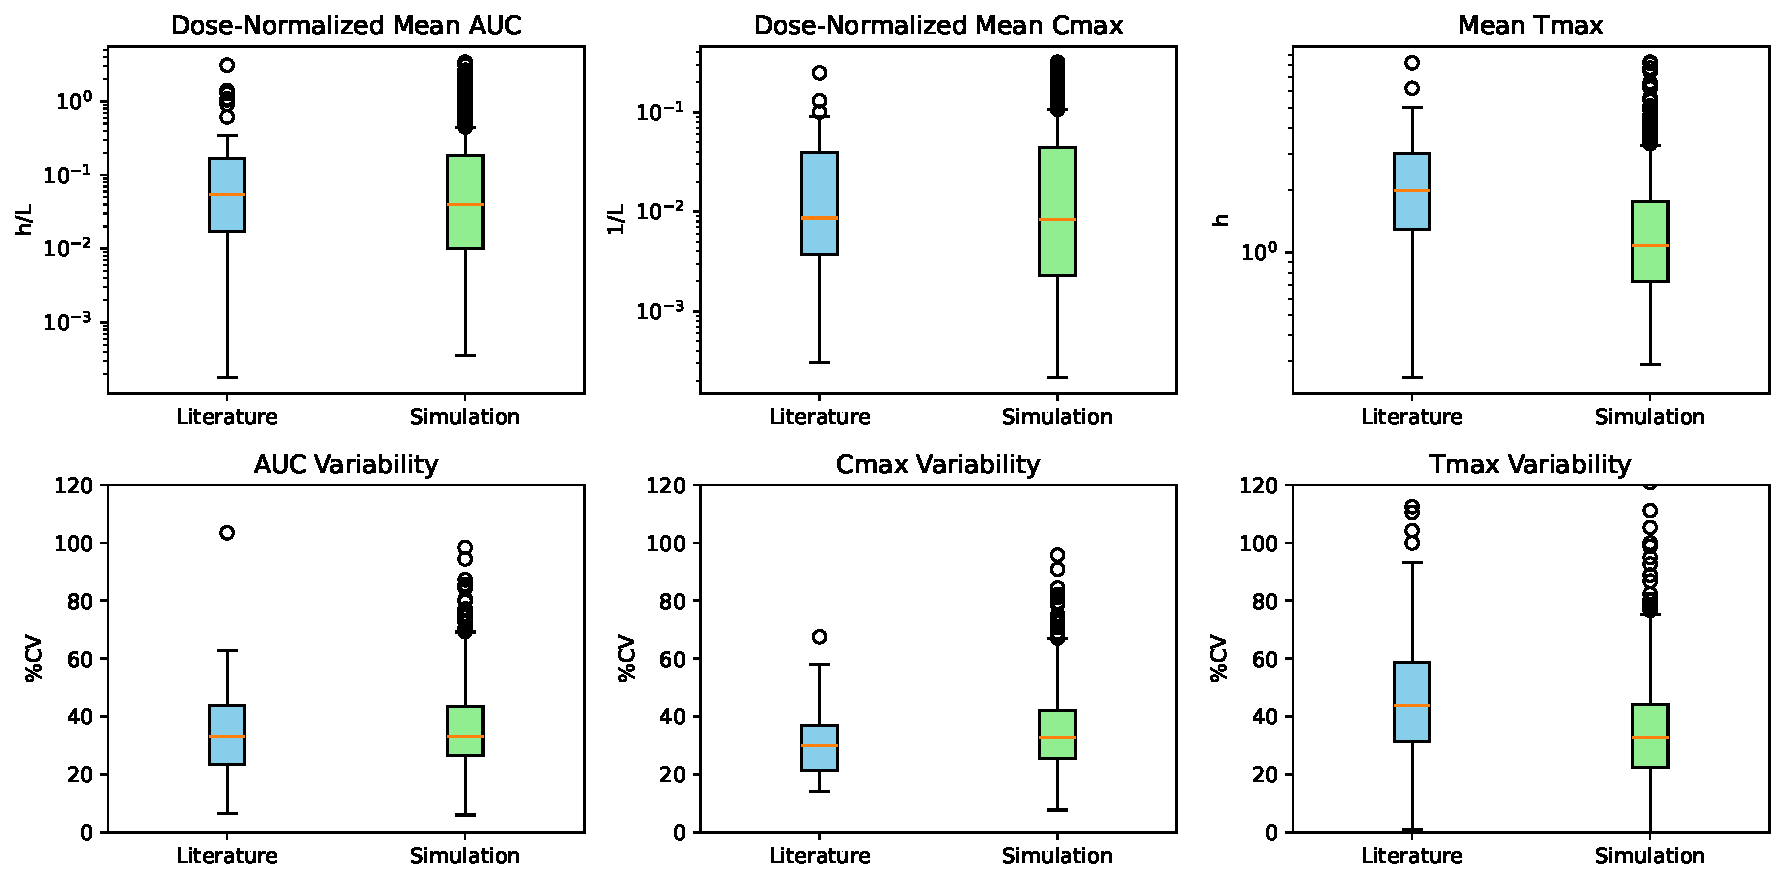
\includegraphics[width=\textwidth]{figures/pk-metrics-literature-vs-simulation.pdf}
    \caption{Comparison of three key PK characteristics (Mean/\%CV) between literature and 1000 simulated datasets.}
    \label{fig:benchmark}
\end{figure}


To ensure machine-readable consistency, we again utilized \texttt{structured outputs} enforced via nested \texttt{Pydantic} models, yielding one JSON record for each paper.
%
Where both fasting and fed-state results were reported, the LLM was instructed to only take fasting values into account.
%
The total API costs for this LLM-based workflow across all 200 screened and 114 classified papers was \$0.31 USD.

\subsection{Post-Processing}
\label{app:postprocessing}

The extracted JSON records were post-processed into a final analysis literature dataset via the following steps:

\begin{itemize}
    \item Amongst the 114 BE trials, we kept only those 85 corresponding to oral administration\footnote{While our framework is capable of simulating intravenous administration as well, a focus on oral dosing allowed for a more meaningful comparison of $C_{\rm max}$ and $T_{\rm max}$};
    \item Units were harmonized across studies and records with incomplete or implausible values (e.g., $T_{\max} > t_\text{last}$ or missing units) were excluded;
    \item $\mathrm{AUC}_{0-t}$ and $C_{\max}$ were dose-normalized;
    \item The dispersion metrics were converted to coefficients of variation (\%CV), which was either directly used if reported or calculated from central tendency and absolute dispersion metrics (using mean/median interchangeably and assuming range=4~SD). 
\end{itemize}

%
The resulting dataset provided empirical reference distributions for dose-normalized $\mathrm{AUC}_{0-t}$, dose-normalized $C_{\max}$ and $T_{\max}$ across a diverse set of compounds and doses, which we used to benchmark the marginal distributions produced by our stochastic generative model.

\subsubsection{Benchmark of data generative model against literature}
\label{app:benchmark}

The parameters of the stochastic data-generating model were matched to the PK metrics obtained from the literature, as shown in Fig.~\ref{fig:benchmark}.


\begin{table}[h]
\centering
\caption{Meta-study configuration parameters used for synthetic PK meta-study generation.}
\label{tab:meta_study_config}
\begin{tabular}{lc}
\toprule
\textbf{Parameter} & \textbf{Value / Range} \\
\midrule

\multicolumn{2}{l}{\textit{Study setup}} \\
\texttt{drug\_id\_options}           & Drug\_A, Drug\_B, Drug\_C \\
\texttt{num\_individuals\_range}     & [5, 10] \\
\texttt{num\_peripherals\_range}     & [1, 3] \\
\texttt{solver\_method}              & rk4 \\

\midrule
\multicolumn{2}{l}{\textit{Time grid}} \\
\texttt{time\_start}                 & 0.0 \\
\texttt{time\_stop}                  & 24.0 \\
\texttt{time\_num\_steps}            & 100 \\

\midrule
\multicolumn{2}{l}{\textit{Absorption parameters ($k_a$)}} \\
\texttt{log\_k\_a\_mean\_range}      & [-1, 2] \\
\texttt{log\_k\_a\_std\_range}       & [0.15, 0.45] \\
\texttt{k\_a\_tmag\_range}           & [0.01, 0.1] \\
\texttt{k\_a\_tscl\_range}           & [1, 5] \\

\midrule
\multicolumn{2}{l}{\textit{Elimination parameters ($k_e$)}} \\
\texttt{log\_k\_e\_mean\_range}      & [-5, 0] \\
\texttt{log\_k\_e\_std\_range}       & [0.15, 0.45] \\
\texttt{k\_e\_tmag\_range}           & [0.01, 0.1] \\
\texttt{k\_e\_tscl\_range}           & [1, 5] \\

\midrule
\multicolumn{2}{l}{\textit{Volume parameters ($V$)}} \\
\texttt{log\_V\_mean\_range}         & [1, 7] \\
\texttt{log\_V\_std\_range}          & [0.15, 0.45] \\
\texttt{V\_tmag\_range}              & [0.001, 0.01] \\
\texttt{V\_tscl\_range}              & [1, 5] \\

\midrule
\multicolumn{2}{l}{\textit{Peripheral exchange ($k_{1p}$)}} \\
\texttt{log\_k\_1p\_mean\_range}     & [-4, 0] \\
\texttt{log\_k\_1p\_std\_range}      & [0.15, 0.45] \\
\texttt{k\_1p\_tmag\_range}          & [0.01, 0.1] \\
\texttt{k\_1p\_tscl\_range}          & [1, 5] \\

\midrule
\multicolumn{2}{l}{\textit{Peripheral return ($k_{p1}$)}} \\
\texttt{log\_k\_p1\_mean\_range}     & [-4, -1] \\
\texttt{log\_k\_p1\_std\_range}      & [0.15, 0.45] \\
\texttt{k\_p1\_tmag\_range}          & [0.01, 0.1] \\
\texttt{k\_p1\_tscl\_range}          & [1, 5] \\

\midrule
\multicolumn{2}{l}{\textit{Observation noise}} \\
\texttt{rel\_ruv\_range}             & [0.01, 0.1] \\

\bottomrule
\end{tabular}
\end{table}
